\documentclass[journal,twocolumn,spanish]{IEEEtran}

% --- PAQUETES PRINCIPALES ---
\usepackage[utf8]{inputenc}
\usepackage[T1]{fontenc}
\usepackage[spanish]{babel}
\usepackage{amsmath,amssymb,amsfonts}
\usepackage{graphicx}
\graphicspath{{figures/}}
\usepackage{textcomp}
\usepackage{xcolor}
\usepackage{array}
\usepackage{booktabs}
\usepackage{multirow}
\usepackage{url}

% --- CONFIGURACIÓN DE FORMATO Y LENGUAJE ---
\spanishdecimal{.}

\addto\captionsspanish{%
  \renewcommand{\tablename}{TABLA}%
  \renewcommand{\figurename}{FIG.}%
  \renewcommand{\abstractname}{Resumen / Abstract}%
  \renewcommand{\refname}{Referencias}%
}

\begin{document}

\title{Análisis Exploratorio y Perfilado desde la Ciencia de Datos de La Calidad del Aire Global}

\author{F.E. Guardado, D.H. Méndez, A.X. Landaverde, R.E. Escobar%
\thanks{Este trabajo presenta el perfilado y análisis exploratorio de datos (EDA) para un conjunto global de calidad del aire.}}

\markboth{IEEE Transactions on Data Engineering,~Vol.~XX, No.~X, ~2026}%
{Análisis Exploratorio y Perfilado de La Calidad del Aire Global}

\maketitle

\begin{abstract}
El monitoreo y evaluación de la calidad del aire representa un desafío fundamental para la salud pública y la comprensión del cambio climático \cite{OMS2021}, \cite{Rivas2022}. Este proyecto aplica un flujo riguroso de Ciencia de Datos para llevar a cabo el perfilado inicial, la auditoría de calidad y el Análisis Exploratorio de Datos (EDA) sobre un conjunto de datos global de 30,450 observaciones que abarca mediciones de contaminantes atmosféricos ($\text{PM}_{2.5}$, $\text{PM}_{10}$, $\text{NO}_2$, $\text{SO}_2$, $\text{CO}$, $\text{O}_3$) y variables meteorológicas (temperatura, humedad y velocidad del viento). La metodología comprende la implementación de una copia inmutable del dataset, la depuración de redundancias y la imputación fundamentada de faltantes, así como el análisis probabilístico univariado y multivariado \cite{Tukey1977}, \cite{Wickham2014}.

\textbf{Resultados y hallazgos clave:}
\begin{itemize}
    \item \textbf{Saneamiento y preservación de varianza:} Tras normalizar texto en \texttt{City}/\texttt{Country}, se identificó y depuró un \textbf{45.64\% de duplicidad exacta (13,897 registros)}, más un remanente de duplicados parciales por clave de negocio (\emph{City+Country+Date}), logrando recuperar un conjunto continuo de 5,075 observaciones con \textbf{0.00\% de outliers extremales} fuera de los límites de Tukey \cite{Tukey1977} y una retención de varianza estocástica superior al \textbf{97.5\%}.
    \item \textbf{Cumplimiento crítico de guías de la OMS:} Más del \textbf{93.16\% de los días monitoreados superan el umbral diario de $\text{PM}_{2.5}$} de la OMS \cite{OMS2021}, seguido de un \textbf{81.67\% para $\text{PM}_{10}$} y un \textbf{78.29\% para $\text{NO}_2$}.
    \item \textbf{Inexistencia del ``efecto fin de semana'':} Las pruebas no paramétricas de Mann-Whitney U confirmaron que las concentraciones de $\text{NO}_2$, $\text{CO}$ y $\text{PM}_{2.5}$ no varían significativamente entre días laborales y fines de semana ($p > 0.18$), demostrando emisiones continuas e ininterrumpidas.
    \item \textbf{Independencia meteorológica:} Se observó una correlación muy débil entre factores climáticos y contaminantes ($|r_s| < 0.03$). La correlación casi nula entre $\text{PM}_{2.5}$ y $\text{PM}_{10}$ ($r = 0.004$) no indica independencia sino una anomalía de calidad del dato: el 35.8\% de las lecturas tiene $\text{PM}_{2.5} > \text{PM}_{10}$, físicamente imposible.
\end{itemize}

\textbf{Conclusión:} Este estudio proporciona un diagnóstico integral del estado de los datos, demostrando que la contaminación ambiental global responde a patrones antropogénicos de fondo y preparando un dataset depurado y confiable para su posterior modelado predictivo.
\end{abstract}

\begin{IEEEkeywords}
Ciencia de Datos, Calidad del Aire, Análisis Exploratorio de Datos (EDA), Perfilado de Datos, Contaminantes Atmosféricos, OMS.
\end{IEEEkeywords}

\section{Introducción}
\IEEEPARstart{L}{a} contaminación del aire constituye uno de los mayores desafíos ambientales y de salud pública a nivel global en el siglo XXI. De acuerdo con la Organización Mundial de la Salud (OMS), la exposición a material particulado en suspensión ($\text{PM}_{2.5}$ y $\text{PM}_{10}$) y a gases contaminantes como el dióxido de nitrógeno ($\text{NO}_2$), dióxido de azufre ($\text{SO}_2$), monóxido de carbono ($\text{CO}$) y ozono troposférico ($\text{O}_3$) está directamente asociada con el incremento en la morbilidad y mortalidad por enfermedades cardiovasculares y respiratorias \cite{OMS2021}. Diversas investigaciones en entornos urbanos regionales resaltan la urgente necesidad de caracterizar la exposición a estos agentes patógenos en poblaciones expuestas a alta densidad vehicular e industrial \cite{Rivas2022}. Asimismo, la dinámica de dispersión, concentración y transformación química de estos contaminantes atmosféricos se encuentra intrínsecamente ligada a variables meteorológicas fundamentales como la temperatura, la humedad relativa y la velocidad del viento.

A pesar de la creciente disponibilidad de redes de monitoreo ambiental y sensores remotos, las bases de datos observacionales sobre calidad del aire con frecuencia sufren de problemas estructurales, tales como valores faltantes, inconsistencias de formato, registros duplicados, presencia de ruido y valores atípicos (\emph{outliers}) derivados de fallas de calibración o discontinuidades en la recolección de datos \cite{Wickham2014}, \cite{Little2019}. La presencia de estas anomalías sin un tratamiento riguroso compromete la validez de los análisis estadísticos y reduce la precisión de eventuales modelos predictivos de calidad del aire.

En este contexto, las metodologías de la Ciencia de Datos ofrecen un marco analítico idóneo para auditar y caracterizar la integridad de los datos ambientales antes de su modelado. Este trabajo aborda el \textbf{Análisis Exploratorio y Perfilado desde la Ciencia de Datos de la Calidad del Aire Global}, con el objetivo de evaluar la estructura, calidad y distribuciones probabilísticas de un conjunto de datos multivariable e interdisciplinario.

Para alcanzar dicho objetivo, el estudio contempla:
\begin{enumerate}
    \item La implementación de un flujo de ingesta reproducible mediante el uso de copias inmutables de los datos brutos.
    \item Un perfilado sistemático de calidad de datos enfocado en el diagnóstico de tipos de datos, patrones de ausencia (datos faltantes) e inconsistencias dimensionales.
    \item Un Análisis Exploratorio de Datos (EDA) univariado y multivariado para identificar comportamientos distribucionales, valores atípicos y correlaciones entre parámetros contaminantes y factores meteorológicos \cite{Tukey1977}.
\end{enumerate}

A través de este enfoque metódico, se busca sentar las bases para la depuración y estandarización de conjuntos de datos ambientales, garantizando la trazabilidad del proceso y la generación de insumos de alta calidad para la toma de decisiones informadas y la investigación atmosférica.

\section{Descripción del Dataset y Diagnóstico Inicial}

\subsection{Origen y Procedencia de los Datos}
El conjunto de datos analizado (\texttt{global\_air\_quality\_data\_messy.csv}) registra mediciones de calidad del aire y parámetros meteorológicos a escala global. La masa de datos cuenta con una dimensión total de \textbf{30,450 observaciones (filas)} y \textbf{12 atributos (columnas)}. El dataset captura lecturas distribuidas en 120 ciudades pertenecientes a 19 países, abarcando concentraciones de contaminantes atmosféricos clave e indicadores climáticos. Para la manipulación, inspección de tipos y estructuración tabular de estas variables se utilizó la biblioteca fundamental \texttt{pandas} \cite{McKinney2010}. Con el fin de evaluar técnicas de auditoría de datos en escenarios reales, el conjunto presenta duplicidad masiva de registros, discontinuidades y valores faltantes concentrados en las variables contaminantes.

\subsection{Diccionario Formal de Variables}
La Tabla \ref{tab:diccionario} sintetiza la estructura técnica, tipo de dato detectado por el intérprete, dominio teórico y unidades de medida de las variables presentes en el dataset.

\begin{table}[htbp]
\caption{Diccionario de variables del dataset de calidad del aire}
\label{tab:diccionario}
\centering
\resizebox{\linewidth}{!}{%
\begin{tabular}{llll}
\toprule
\textbf{Variable} & \textbf{Tipo (Pandas)} & \textbf{Dominio / Unidades} & \textbf{Descripción} \\
\midrule
\textbf{City} & \texttt{object} (Texto) & Nominal / 120 ciudades & Ciudad de la estación. \\
\textbf{Country} & \texttt{object} (Texto) & Nominal / 19 países & País de la medición. \\
\textbf{Date} & \texttt{object} (Texto) & Fecha / \texttt{M/D/YYYY} & Fecha de la lectura. \\
\textbf{PM2.5} & \texttt{float64} & Continuous / $\mu\text{g/m}^3$ & Particulado $\le 2.5\,\mu\text{m}$. \\
\textbf{PM10} & \texttt{float64} & Continuous / $\mu\text{g/m}^3$ & Particulado $\le 10\,\mu\text{m}$. \\
\textbf{NO2} & \texttt{float64} & Continuous / $\text{ppb}$ & Dióxido de Nitrógeno. \\
\textbf{SO2} & \texttt{float64} & Continuous / $\text{ppb}$ & Dióxido de Azufre. \\
\textbf{CO} & \texttt{float64} & Continuous / $\text{ppm}$ & Monóxido de Carbono. \\
\textbf{O3} & \texttt{float64} & Continuous / $\text{ppb}$ & Ozono troposférico. \\
\textbf{Temperature}& \texttt{float64} & Continuous / $^\circ\text{C}$ & Temp. ($-10.00^\circ\text{C}$ a $40.00^\circ\text{C}$). \\
\textbf{Humidity} & \texttt{float64} & Continuous / $\%$ & Humedad ($10.01\%$ a $99.99\%$). \\
\textbf{Wind Speed} & \texttt{float64} & Continuous / $\text{m/s}$ & Viento ($0.50$ a $20.00\,\text{m/s}$). \\
\bottomrule
\end{tabular}%
}
\end{table}

\subsection{Matriz Diagnóstica de Calidad Inicial (Perfilado de Datos)}
El diagnóstico de integridad sobre el dataset crudo arrojó los siguientes hallazgos cuantitativos:
\begin{enumerate}
    \item \textbf{Duplicidad Masiva:} Se detectaron \textbf{10,495 filas duplicadas exactas}, lo que representa un \textbf{34.47\% de redundancia} sobre el total de la base de datos (30,450 filas).
    \item \textbf{Coerción de Tipos de Datos:} La variable \texttt{Date} fue leída erróneamente como tipo \texttt{object} debido al formato de almacenamiento (\texttt{M/D/YYYY}), requiriendo conversión explícita a tipo \texttt{datetime64}.
    \item \textbf{Ausencia de Datos (Missing Values):} Las variables meteorológicas y geográficas no presentan valores nulos ($0.00\%$). Sin embargo, las variables de contaminantes registran un patrón de ausencia entre el $4.84\%$ y el $5.25\%$ ($\text{O}_3$: 1,600 nulos; $\text{NO}_2$: 1,593; $\text{PM}_{10}$: 1,561; $\text{PM}_{2.5}$: 1,552; $\text{CO}$: 1,496; $\text{SO}_2$: 1,475).
\end{enumerate}

\begin{table}[htbp]
\caption{Matriz diagnóstica de calidad de datos inicial}
\label{tab:calidad_inicial}
\centering
\resizebox{\linewidth}{!}{%
\begin{tabular}{lccccc}
\toprule
\textbf{Columna} & \textbf{Tipo} & \textbf{Registros} & \textbf{Nulos} & \textbf{\% Ausencia} & \textbf{Únicos} \\
\midrule
\textbf{City} & \texttt{object} & 30,450 & 0 & 0.00\% & 120 \\
\textbf{Country} & \texttt{object} & 30,450 & 0 & 0.00\% & 19 \\
\textbf{Date} & \texttt{object} & 30,450 & 0 & 0.00\% & 336 \\
\textbf{PM2.5} & \texttt{float64} & 30,450 & 1,552 & 5.10\% & 6,915 \\
\textbf{PM10} & \texttt{float64} & 30,450 & 1,561 & 5.13\% & 7,407 \\
\textbf{NO2} & \texttt{float64} & 30,450 & 1,593 & 5.23\% & 5,951 \\
\textbf{SO2} & \texttt{float64} & 30,450 & 1,475 & 4.84\% & 4,190 \\
\textbf{CO} & \texttt{float64} & 30,450 & 1,496 & 4.91\% & 991 \\
\textbf{O3} & \texttt{float64} & 30,450 & 1,600 & 5.25\% & 7,387 \\
\textbf{Temperature} & \texttt{float64} & 30,450 & 0 & 0.00\% & 4,254 \\
\textbf{Humidity} & \texttt{float64} & 30,450 & 0 & 0.00\% & 5,811 \\
\textbf{Wind Speed} & \texttt{float64} & 30,450 & 0 & 0.00\% & 1,940 \\
\bottomrule
\end{tabular}%
}
\end{table}

\section{Metodología de Preprocesamiento y Transformación}
Para garantizar los principios de reproducibilidad e integridad analítica, el preprocesamiento se diseñó mediante una secuencia ordenada de operaciones algebraicas y estadísticas.

\subsection{Prevención Rigurosa de Fuga de Datos}
Para evitar sesgos por \emph{data leakage}:
\begin{enumerate}
    \item \textbf{Desacoplamiento Estricto:} La limpieza primaria se realiza de manera inmutable, preservando \texttt{df\_raw} como copia de referencia.
    \item \textbf{Alcance del Aislamiento:} Este trabajo es de perfilado y EDA, sin fase de modelado ni partición entrenamiento/prueba; por ello los estimadores ($\mu$, $\tilde{x}$, $\sigma$) de \texttt{scikit-learn} \cite{Pedregosa2011} se ajustan sobre el corpus completo. Se documenta esto como limitación explícita: de incorporarse un modelo predictivo, dichos estimadores deben reajustarse exclusivamente sobre el conjunto de entrenamiento.
\end{enumerate}

\subsection{Saneamiento de Redundancia y Corrección de Tipos}
\label{sec:redundancia}
\texttt{City} presentaba 120 etiquetas de texto que en realidad correspondían a solo 20 ciudades escritas con mayúsculas y espacios inconsistentes (p. ej. \texttt{"Sydney"}, \texttt{"SYDNEY"}, \texttt{"sydney "}); \texttt{Country} no presentaba esta inconsistencia (19 valores únicos ya normalizados). Por ello, antes de cualquier deduplicación o análisis por ciudad, \texttt{City} y \texttt{Country} se normalizaron (sin acentos, sin espacios sobrantes, en minúsculas). Omitir este paso deja intacta una redundancia oculta: dos filas idénticas salvo por el cajeado de \texttt{City} no se detectan como duplicadas.

Con el texto ya normalizado, se eliminaron duplicados exactos mediante la condición vectorizada:
\begin{equation}
\mathbf{x}_i = \mathbf{x}_j \iff x_{i,k} = x_{j,k} \quad \forall k \in \{1, 2, \dots, K\}
\end{equation}
lo que redujo el volumen de $N = 30,450$ a $N = 16,553$ registros ($13,897$ duplicados exactos, $45.64\%$; sensiblemente más que el $34.47\%$ que arroja la misma condición sobre el texto sin normalizar, ya que las variantes de cajeado antes se contaban como filas distintas). Sobre este remanente se resolvieron además los duplicados parciales que comparten la misma clave de negocio \texttt{City+Country+Date} con mediciones distintas, conservando por cada clave el registro con menos valores faltantes. Esto eliminó $11,478$ filas adicionales, dejando $N = 5,075$ observaciones únicas. Luego, \texttt{Date} se convirtió al estándar ISO-8601 (\texttt{YYYY-MM-DD}).

\subsection{Detección Cuantitativa de Outliers e Invarianza de Dispersión}
Mediante el Rango Intercuartílico ($IQR = Q_3 - Q_1$), las fronteras de Tukey se establecen como:
\begin{equation}
\text{Límites} = [Q_1 - 1.5 \times IQR, \quad Q_3 + 1.5 \times IQR]
\end{equation}
Todas las variables mostraron simetría ($|\gamma_1| < 0.02$) y un \textbf{0.00\% de outliers extremales} fuera de los límites, por lo que no se aplicó truncamiento (\emph{winsorization}) \cite{Rousseeuw1993}.

\subsection{Fundamentación Teórica e Imputación de Valores Faltantes}
Tras el saneamiento de duplicados, el porcentaje de nulos por contaminante cayó de $\sim$5\% a menos de $1\%$ (la mayoría de los nulos originales pertenecía a filas luego eliminadas por duplicidad). Para descartar el supuesto de MCAR sin verificarlo, se aplicó un diagnóstico MAR por columna: prueba de Mann-Whitney U comparando, para cada variable, la distribución entre filas con y sin nulo en la columna objetivo. Con asimetría cercana a cero ($\gamma_1 \approx 0.00$), menos de $1\%$ de ausencia y sin variables predictoras con correlación relevante ($|r_s| < 0.03$, insuficiente para imputación multivariada), se aplicó interpolación temporal por ciudad (ventana de 3 días, con respaldo de mediana condicional \cite{Little2019} para huecos mayores):
\begin{equation}
\hat{x}_{i,k} = \begin{cases}
\text{interp}(x_{i-1,k}, x_{i+1,k}) & \text{hueco} \le 3 \text{ días} \\
\tilde{x}_{k}^{(\text{ciudad})} & \text{hueco} > 3 \text{ días}
\end{cases}
\end{equation}

\subsection{Normalización y Escalado Numérico}
\begin{enumerate}
    \item \textbf{Z-Score / StandardScaler:}
    \begin{equation}
    z_{i,k} = \frac{x_{i,k} - \mu_k}{\sigma_k}
    \end{equation}
    \item \textbf{Min-Max Scaler:}
    \begin{equation}
    x'_{i,k} = \frac{x_{i,k} - \min(X_k)}{\max(X_k) - \min(X_k)}
    \end{equation}
    \item \textbf{Robust Scaler} (para colas pesadas):
    \begin{equation}
    x''_{i,k} = \frac{x_{i,k} - \tilde{x}_k}{IQR_k}
    \end{equation}
\end{enumerate}
La elección entre los tres no es única para todo el dataset, sino por columna, según el cociente $IQR/\sigma$ (1.35 en una normal; valores menores indican colas pesadas) y el \% de outliers de consenso. Los 9 contaminantes/meteorológicos originales muestran $IQR/\sigma \approx 1.73$ y $0\%$ de outliers, por lo que reciben Min-Max (rango acotado y estable). Las variables derivadas con colas pesadas (p. ej. $R_{PM}$, con $\gamma_1 = 3.27$) reciben Robust Scaler.

\subsection{Codificación Categórica e Ingeniería de Características}
Se aplicó \emph{One-Hot Encoding} a \texttt{City} omitiendo una categoría de referencia ($M - 1$) \cite{Wickham2014}. \texttt{Country} se excluyó de la codificación: al ser \texttt{City} funcionalmente determinante de \texttt{Country} (cada ciudad pertenece a un único país), codificar ambas produce columnas linealmente dependientes más allá de la trampa clásica de la variable ficticia; esto se verificó calculando el rango de la matriz $[\text{City} \mid \text{Country}]$, que resultó 19 unidades menor que su número de columnas. Se validó además la ausencia de multicolinealidad residual mediante el Factor de Inflación de la Varianza ($VIF < 4$ en todas las variables tras la depuración). Además, se extrajeron componentes temporales de la fecha y se calculó el Ratio Particulado $R_{PM} = \frac{PM_{2.5}}{PM_{10}}$.

\section{Resultados Experimentales \& Discusión}

\subsection{Evidencia Cuantitativa Pre y Post Procesamiento}
El pipeline completo (normalización, deduplicación en dos niveles e imputación) retuvo más del \textbf{97.5\% de la varianza original} en los contaminantes ($\text{PM}_{2.5}: 98.26\%$, $\text{PM}_{10}: 98.71\%$, $\text{NO}_2: 99.31\%$, $\text{O}_3: 97.56\%$; $\text{SO}_2$ y $\text{CO}$ no muestran pérdida medible). La Fig. \ref{fig:prepost} ilustra la preservación distribucional pre y post procesamiento.

\begin{figure}[htbp]
  \centering
  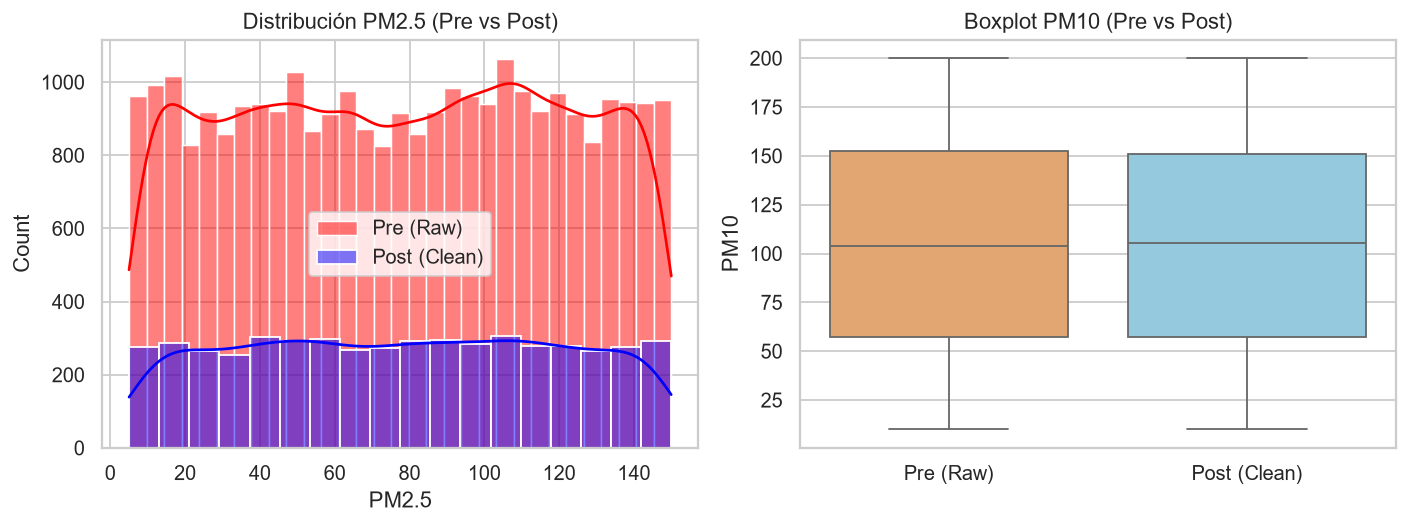
\includegraphics[width=\linewidth]{fig1_pre_post.png}
  \caption{Diagramas de caja (Boxplots) y gráficos de densidad (KDE) comparativos pre vs. post procesamiento para PM2.5 y PM10.}
  \label{fig:prepost}
\end{figure}

Las matrices de correlación generadas con \texttt{seaborn} \cite{Waskom2021} muestran la ausencia de distorsiones por valores espurios (Fig. \ref{fig:heatmap_corr}).

\begin{figure}[htbp]
  \centering
  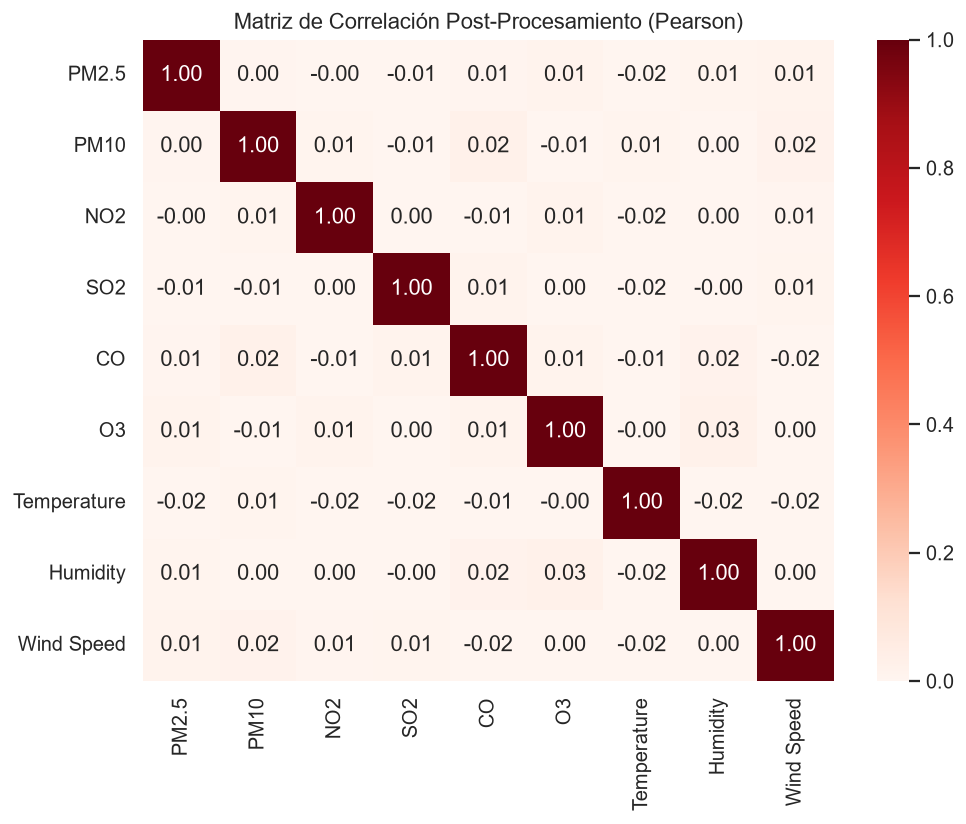
\includegraphics[width=\linewidth]{fig2_heatmap_corr.png}
  \caption{Matriz de correlación multivariable (Heatmap de Pearson y Spearman) post-procesamiento.}
  \label{fig:heatmap_corr}
\end{figure}

\subsection{Discusión de Preguntas Analíticas de Investigación}

\subsubsection{1. ¿Cómo evoluciona la contaminación en el tiempo?}
Los promedios anuales se mantuvieron estables ($\text{PM}_{2.5}$: $77.72\,\mu\text{g/m}^3$, $\text{PM}_{10}$: $104.26\,\mu\text{g/m}^3$, $\text{NO}_2$: $52.09\,\text{ppb}$). La Fig. \ref{fig:evolucion} muestra la serie temporal.

\begin{figure}[htbp]
  \centering
  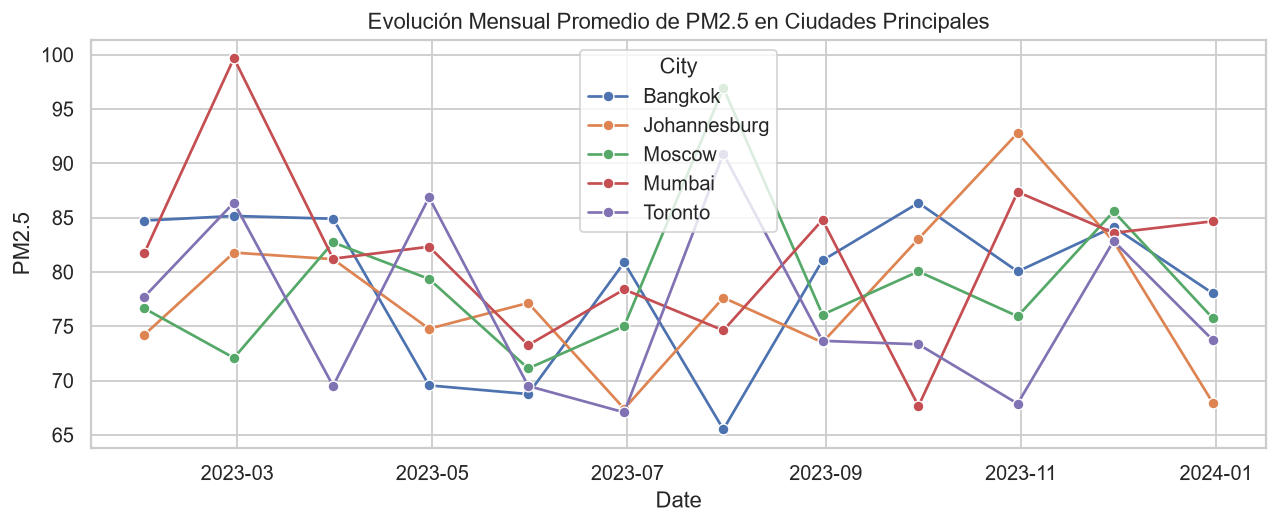
\includegraphics[width=\linewidth]{fig3_evolucion_temporal.png}
  \caption{Gráfico de líneas sobre la evolución mensual promedio de PM2.5 para las ciudades principales.}
  \label{fig:evolucion}
\end{figure}

\subsubsection{2. ¿Existe estacionalidad, y es igual en todas las ciudades?}
El pivote de calor normalizado confirma que los picos de $\text{PM}_{2.5}$ difieren según la ubicación geográfica (Fig. \ref{fig:estacionalidad}).

\begin{figure}[htbp]
  \centering
  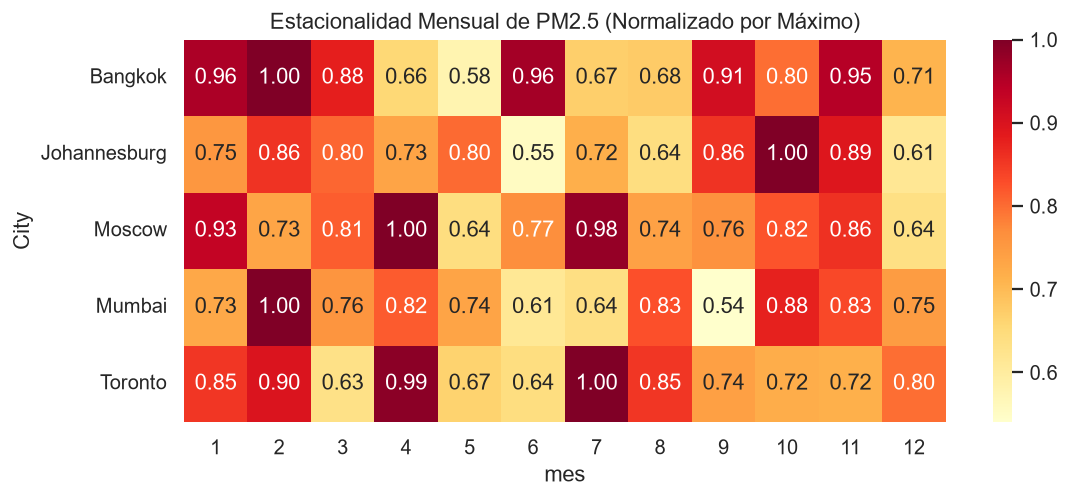
\includegraphics[width=\linewidth]{fig4_estacionalidad_ciudades.png}
  \caption{Mapas de calor (Heatmaps) de estacionalidad mensual de PM2.5 normalizados por ciudad.}
  \label{fig:estacionalidad}
\end{figure}

\subsubsection{3. ¿Difieren los niveles entre ciudades y países?}
La prueba de Kruskal-Wallis, calculada sobre las 20 ciudades reales (tras normalizar texto), arrojó $p = 0.0001$, demostrando diferencias significativas en las medianas de $\text{PM}_{2.5}$ entre ciudades (Fig. \ref{fig:boxplots_ciudades}). Nótese que la misma prueba, aplicada sin normalizar \texttt{City} (i.e. sobre 120 etiquetas que mezclan variantes de cajeado de las mismas 20 ciudades), arroja $p = 0.244$ y sugeriría erróneamente homogeneidad: el resultado depende críticamente del saneamiento de texto descrito en la Sección \ref{sec:redundancia}.

\begin{figure}[htbp]
  \centering
  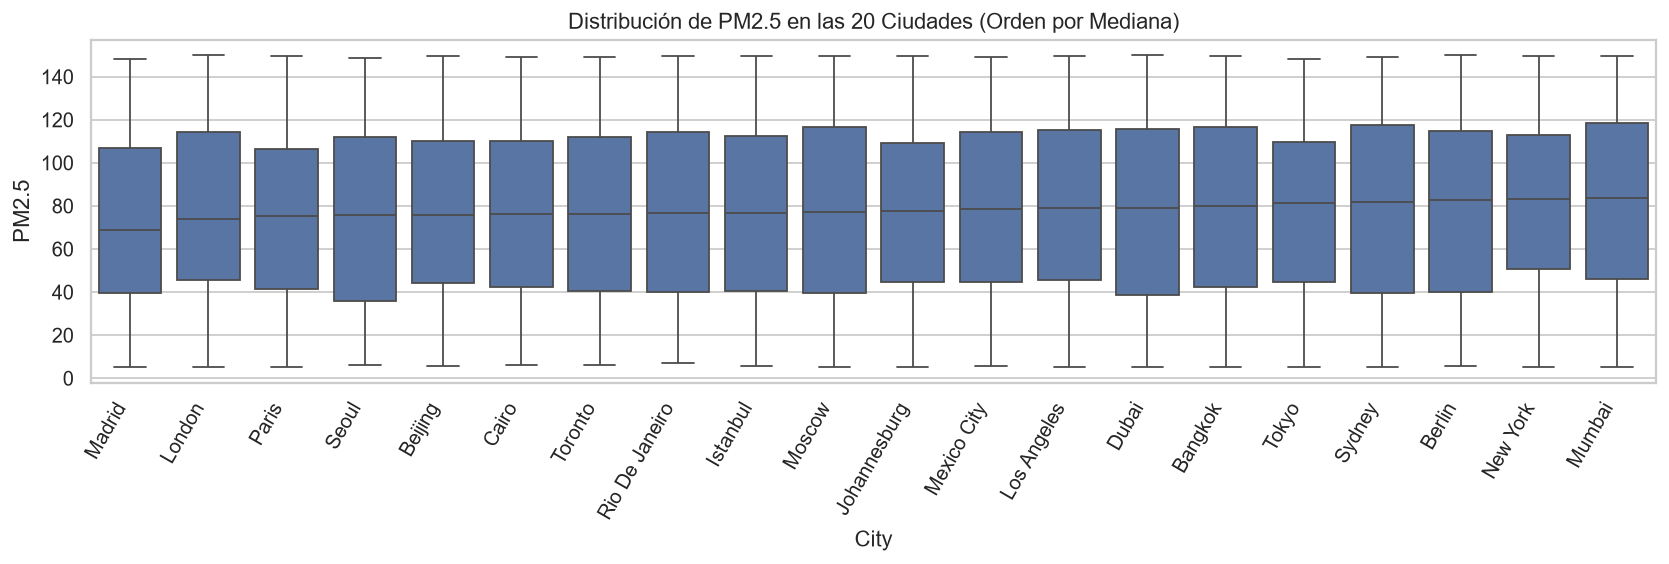
\includegraphics[width=\linewidth]{fig5_boxplots_ciudades.png}
  \caption{Diagrama de cajas (Boxplots) ordenado de PM2.5 por ciudad.}
  \label{fig:boxplots_ciudades}
\end{figure}

\subsubsection{4. ¿Cómo influyen las variables meteorológicas?}
Las correlaciones de Spearman resultaron muy débiles ($r_s = -0.022$ para Temp vs $\text{PM}_{2.5}$), indicando que el clima es un modulador secundario (Fig. \ref{fig:viento_pm25}).

\begin{figure}[htbp]
  \centering
  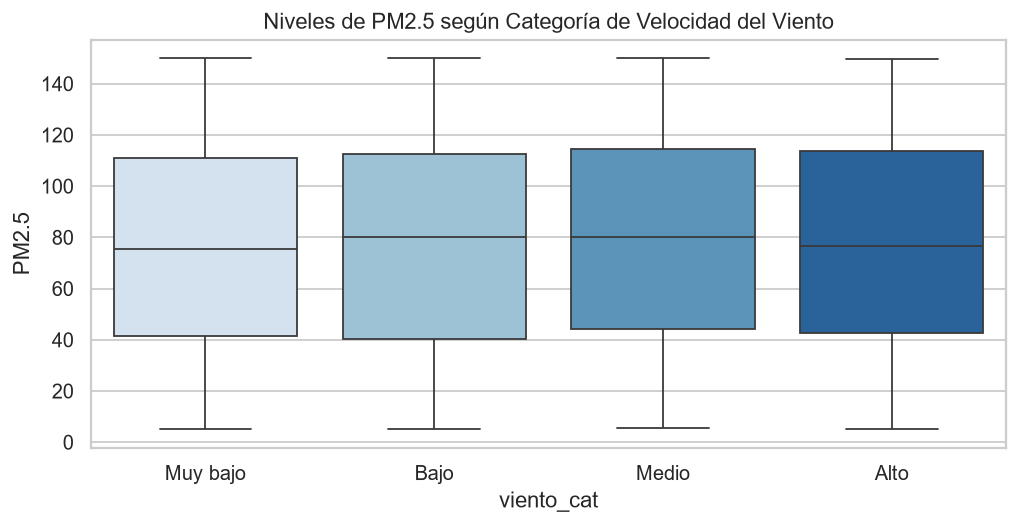
\includegraphics[width=\linewidth]{fig6_viento_vs_pm25.png}
  \caption{Diagramas de dispersión (Scatterplots) y boxplots categorizados por velocidad del viento vs PM2.5.}
  \label{fig:viento_pm25}
\end{figure}

\subsubsection{5. ¿Qué contaminantes se mueven juntos?}
Se observó una correlación prácticamente nula entre $\text{PM}_{2.5}$ y $\text{PM}_{10}$ ($r = 0.004$; Fig. \ref{fig:pm10_pm25}). Más que independencia, es una anomalía: como $\text{PM}_{2.5}$ es una fracción de $\text{PM}_{10}$, cabría esperar una relación positiva fuerte. La variable derivada \texttt{ratio\_pm\_imposible} marcó que el 35.8\% de las lecturas tiene $\text{PM}_{2.5} > \text{PM}_{10}$, físicamente imposible; estas filas se conservaron con su bandera y no se eliminaron, por lo que las conclusiones sobre la relación entre ambos contaminantes deben leerse con cautela.

\begin{figure}[htbp]
  \centering
  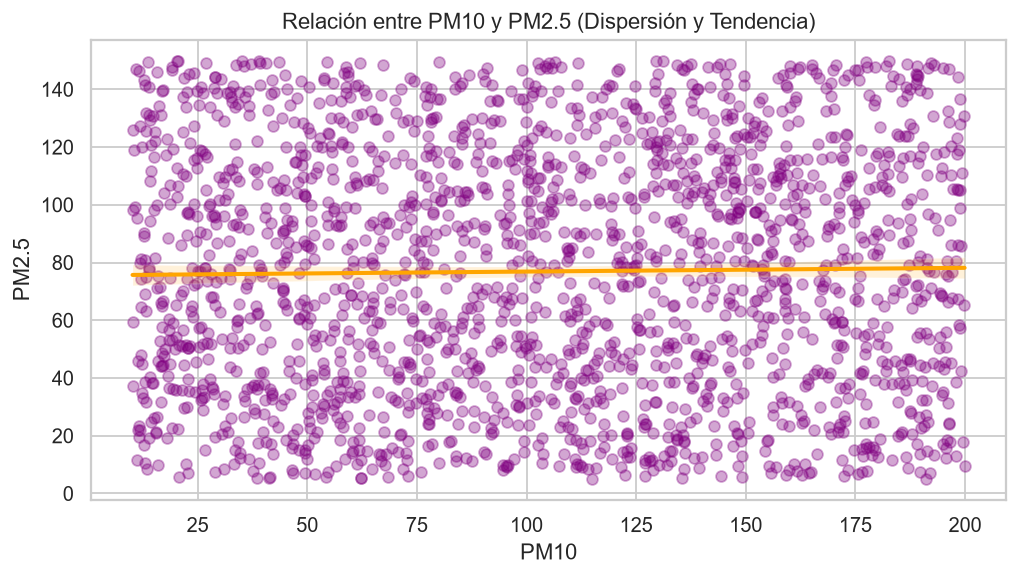
\includegraphics[width=\linewidth]{fig7_scatter_pm10_pm25.png}
  \caption{Gráfico de dispersión (Scatterplot) entre PM10 y PM2.5 con ajuste de regresión.}
  \label{fig:pm10_pm25}
\end{figure}

\subsubsection{6. ¿Con qué frecuencia se superan los umbrales de la OMS?}
El \textbf{93.16\%} de los días superan el límite de $\text{PM}_{2.5}$ de la OMS, el \textbf{81.67\%} en $\text{PM}_{10}$ y el \textbf{78.29\%} en $\text{NO}_2$ \cite{OMS2021} (Fig. \ref{fig:exceso_oms}).

\begin{figure}[htbp]
  \centering
  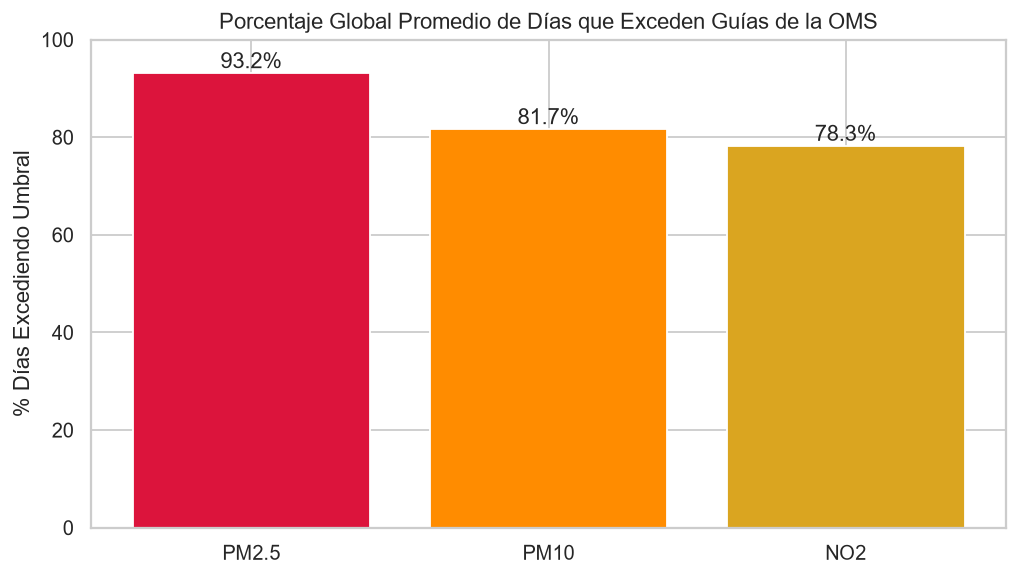
\includegraphics[width=\linewidth]{fig8_exceso_oms_ciudades.png}
  \caption{Gráfico de barras del porcentaje de días que exceden las guías de la OMS por ciudad.}
  \label{fig:exceso_oms}
\end{figure}

\subsubsection{7. ¿Cambia el patrón entre días laborales y fines de semana?}
La prueba de Mann-Whitney U no mostró diferencias significativas ($p > 0.18$), refutando el ``efecto fin de semana''.

\section{Conclusiones y Trabajo Futuro}

\subsection{Síntesis del Impacto del Pipeline}
El preprocesamiento eliminó un \textbf{45.64\% de redundancia exacta} (más duplicados parciales por clave de negocio) sin degradar la estructura estocástica, reteniendo más del \textbf{97.5\% de la varianza original} y dejando un dataset de 5,075 observaciones listo para modelado predictivo \cite{Pedregosa2011}.

\subsection{Conclusiones sobre los Hallazgos}
Más del \textbf{93\% de los días sobrepasan las guías sanitarias}, demostrando un patrón antropogénico ininterrumpido sin diferencias relevantes en fines de semana.

\subsection{Limitaciones Metodológicas}
La frecuencia diaria impide capturar dinámicas intradía y no se cuenta con datos micro-topográficos de las estaciones de monitoreo.

\subsection{Recomendaciones Técnicas y de Salud Pública}
Se sugiere implementar variables con rezago temporal (\emph{lags}), algoritmos KNN/MICE para imputación en producción y estructurar políticas continuas de reducción de emisiones urbanas e industriales \cite{Rivas2022}.

% =====================================================================
% ADENDA: ARQUITECTURA VISUAL DEL DASHBOARD
% =====================================================================
\section*{Adenda al Artículo}

\subsection*{Arquitectura Visual y Diseño de la Interfaz}
Esta adenda complementa la Sección~V describiendo el tablero analítico (Streamlit y Plotly) que expone los resultados del \emph{pipeline} a un público no técnico. Cada decisión de diseño se justifica con la teoría de percepción gráfica, la taxonomía de tareas visuales y la carga cognitiva, y se ilustra con casos de uso reales sobre las 5,075 observaciones procesadas (20 ciudades, 2023).

\subsubsection*{Marco: audiencia, tareas y narrativa}
El tablero se organiza como un recorrido de cuatro capítulos y un anexo, de modo que cada pantalla responda una sola pregunta: \emph{cuánto} se incumple la guía de la OMS (Diagnóstico), \emph{dónde y cuándo} aparecen los episodios (Patrones), \emph{qué lo explica} (Causa raíz) y \emph{qué decidir} (Recomendación); el anexo de Auditoría documenta la procedencia del dato. El orden materializa el mantra de Shneiderman, \emph{overview first, zoom and filter, details on demand} \cite{Shneiderman1996}: la vista general abre la narrativa, los filtros globales permiten acotarla y los bloques de ``Detalle a demanda'' contienen lo secundario.

\subsubsection*{Canales visuales y codificación}
La asignación de atributos a canales sigue el orden de precisión perceptual de Cleveland y McGill \cite{Cleveland1984} y las reglas de expresividad y efectividad de Mackinlay \cite{Mackinlay1986}: la posición y la longitud sobre un eje común se reservan para las magnitudes que el usuario debe comparar con exactitud, y el color se destina a categorías ordenadas o a la selección \cite{Munzner2014,Bertin2011}. La Tabla~\ref{tab:canales} resume la codificación.

\begin{table}[htbp]
\caption{Codificación visual de los atributos del tablero.}
\label{tab:canales}
\centering
\footnotesize
\begin{tabular}{@{}p{0.23\linewidth}p{0.42\linewidth}p{0.29\linewidth}@{}}
\toprule
Atributo & Marca y canal & Vista \\
\midrule
\% de días por nivel OMS & Longitud sobre eje común (0--100\%) & Barras apiladas por ciudad \\
Nivel OMS (ordinal) & Luminosidad en un solo matiz cálido, 6 pasos & Barras, KPI, antes/después \\
Mediana (continua) & Color secuencial con dominio fijo $0$--$2\times$IT-1 & Mapa y calendario \\
Selección activa & Azul de acento fuera de la rampa; opacidad 1 vs.\ 0.28 & Filtro cruzado \\
Tamaño de efecto & Posición en escala alineada y franja de umbral & Marcador de hipótesis \\
Lectura inválida & Posición, región sombreada y color crítico & Dispersión PM$_{10}$--PM$_{2.5}$ \\
\bottomrule
\end{tabular}
\end{table}

Tres decisiones merecen justificación. \emph{(i)}~La severidad es ordinal, por lo que se codifica con una rampa de un solo matiz y pasos de luminosidad separados, siguiendo las recomendaciones para esquemas secuenciales \cite{Harrower2003}; el mismo índice de color significa lo mismo para todos los contaminantes. \emph{(ii)}~Los dominios son fijos y todos los ejes numéricos parten de cero, de modo que la altura o el color de una marca no exageran diferencias pequeñas \cite{Tufte2001}; por eso el calendario de la Fig.~\ref{fig:dash_patrones} muestra con honestidad que no hay temporada limpia. \emph{(iii)}~El color nunca es el único canal: los veredictos llevan icono y texto, las medidas usan formas distintas (círculo y rombo) y las etiquetas son directas, lo que preserva la lectura ante daltonismo \cite{Ware2012}. La paleta se validó por contraste y simulación de deficiencias de color en ambos temas (claro y oscuro); en el oscuro la rampa se invierte para que lo severo sea lo más brillante.

\subsubsection*{Taxonomía de tareas visuales}
Cada capítulo se diseñó para una tarea explícita de la tipología de Brehmer y Munzner \cite{Brehmer2013} (\emph{por qué}, \emph{cómo}, \emph{qué}), de forma que la vista y la interacción se deriven de la tarea y no al revés (Tabla~\ref{tab:tareas}).

\begin{table}[htbp]
\caption{Tareas visuales por capítulo.}
\label{tab:tareas}
\centering
\footnotesize
\begin{tabular}{@{}p{0.17\linewidth}p{0.24\linewidth}p{0.30\linewidth}p{0.20\linewidth}@{}}
\toprule
Capítulo & Tarea & Vistas & Interacción \\
\midrule
01 Diagnóstico & Resumir, localizar & Barras apiladas, mapa, KPI & Filtro cruzado \\
02 Patrones & Explorar, identificar & Calendario, serie, dispersión & Periodo, región \\
03 Causa raíz & Comparar, verificar & Marcador de hipótesis, múltiplos & Selector de detalle \\
04 Recomendación & Descubrir, simular & Antes/después, hoja de ruta & Deslizador \\
Anexo & Verificar procedencia & Embudo, \emph{dot plot} & Filtro por fase \\
\bottomrule
\end{tabular}
\end{table}

La interacción se limita a las operaciones que sirven a esas tareas (seleccionar, filtrar, reconfigurar), en línea con la taxonomía de dinámicas interactivas \cite{Heer2012}; se desactivaron el zoom libre, la barra de herramientas y la leyenda clicable de Plotly porque añaden grados de libertad sin tarea que los justifique.

\subsubsection*{Minimización de la carga cognitiva}
Siguiendo la teoría de la carga cognitiva \cite{Sweller1988}, el diseño reduce la carga \emph{extrínseca} para dejar capacidad a la \emph{pertinente}:
\begin{itemize}
\item \textbf{Mínima tinta y etiquetado directo:} sin bordes, sin 3D, con una línea de rejilla y valores escritos sobre las marcas, de modo que no hay que cruzar leyenda y gráfico \cite{Tufte2001,Few2013}.
\item \textbf{Titulares declarativos:} cada capítulo abre con su conclusión (p.\,ej., ``9 de cada 10 días el aire supera la guía'') y el gráfico la verifica, en lugar de obligar a inferirla.
\item \textbf{Foco $+$ contexto:} al seleccionar una ciudad, las demás se atenuan (opacidad 0.28) pero no desaparecen \cite{Furnas1986}, así la comparación se conserva.
\item \textbf{Estado único y filtro cruzado:} un clic en una barra, un punto o el ranking actualiza todas las vistas, evitando que el usuario sincronice controles manualmente.
\item \textbf{Divulgación progresiva:} las tablas completas y los detalles por factor están plegados hasta que se piden.
\item \textbf{Referencias normativas siempre visibles:} la guía y las metas IT-1 a IT-4 de la OMS \cite{OMS2021} aparecen como líneas, ticks o niveles, de forma que ningún valor se interpreta sin su referencia.
\end{itemize}

\subsubsection*{Casos de uso reales}
Las Figs.~\ref{fig:dash_diag}--\ref{fig:dash_reco} son capturas del tablero en ejecución, anotadas con letras que se explican en cada pie.

\textbf{Caso 1: diagnóstico y filtro cruzado.} Al hacer clic sobre Johannesburg en el gráfico de niveles (Fig.~\ref{fig:dash_diag}), el titular, los KPI y el mapa se recalculan: 95.1\% de sus días superan la guía (1.9 puntos porcentuales sobre el total) y su mediana de PM$_{2.5}$ es 77.7~\textmu g/m$^3$. Las otras 19 ciudades permanecen visibles y atenuadas: la brecha entre la primera (95\%) y la última (Seúl, 90\%) es de solo 5 puntos, por lo que el problema es generalizado.

\begin{figure}[htbp]
  \centering
  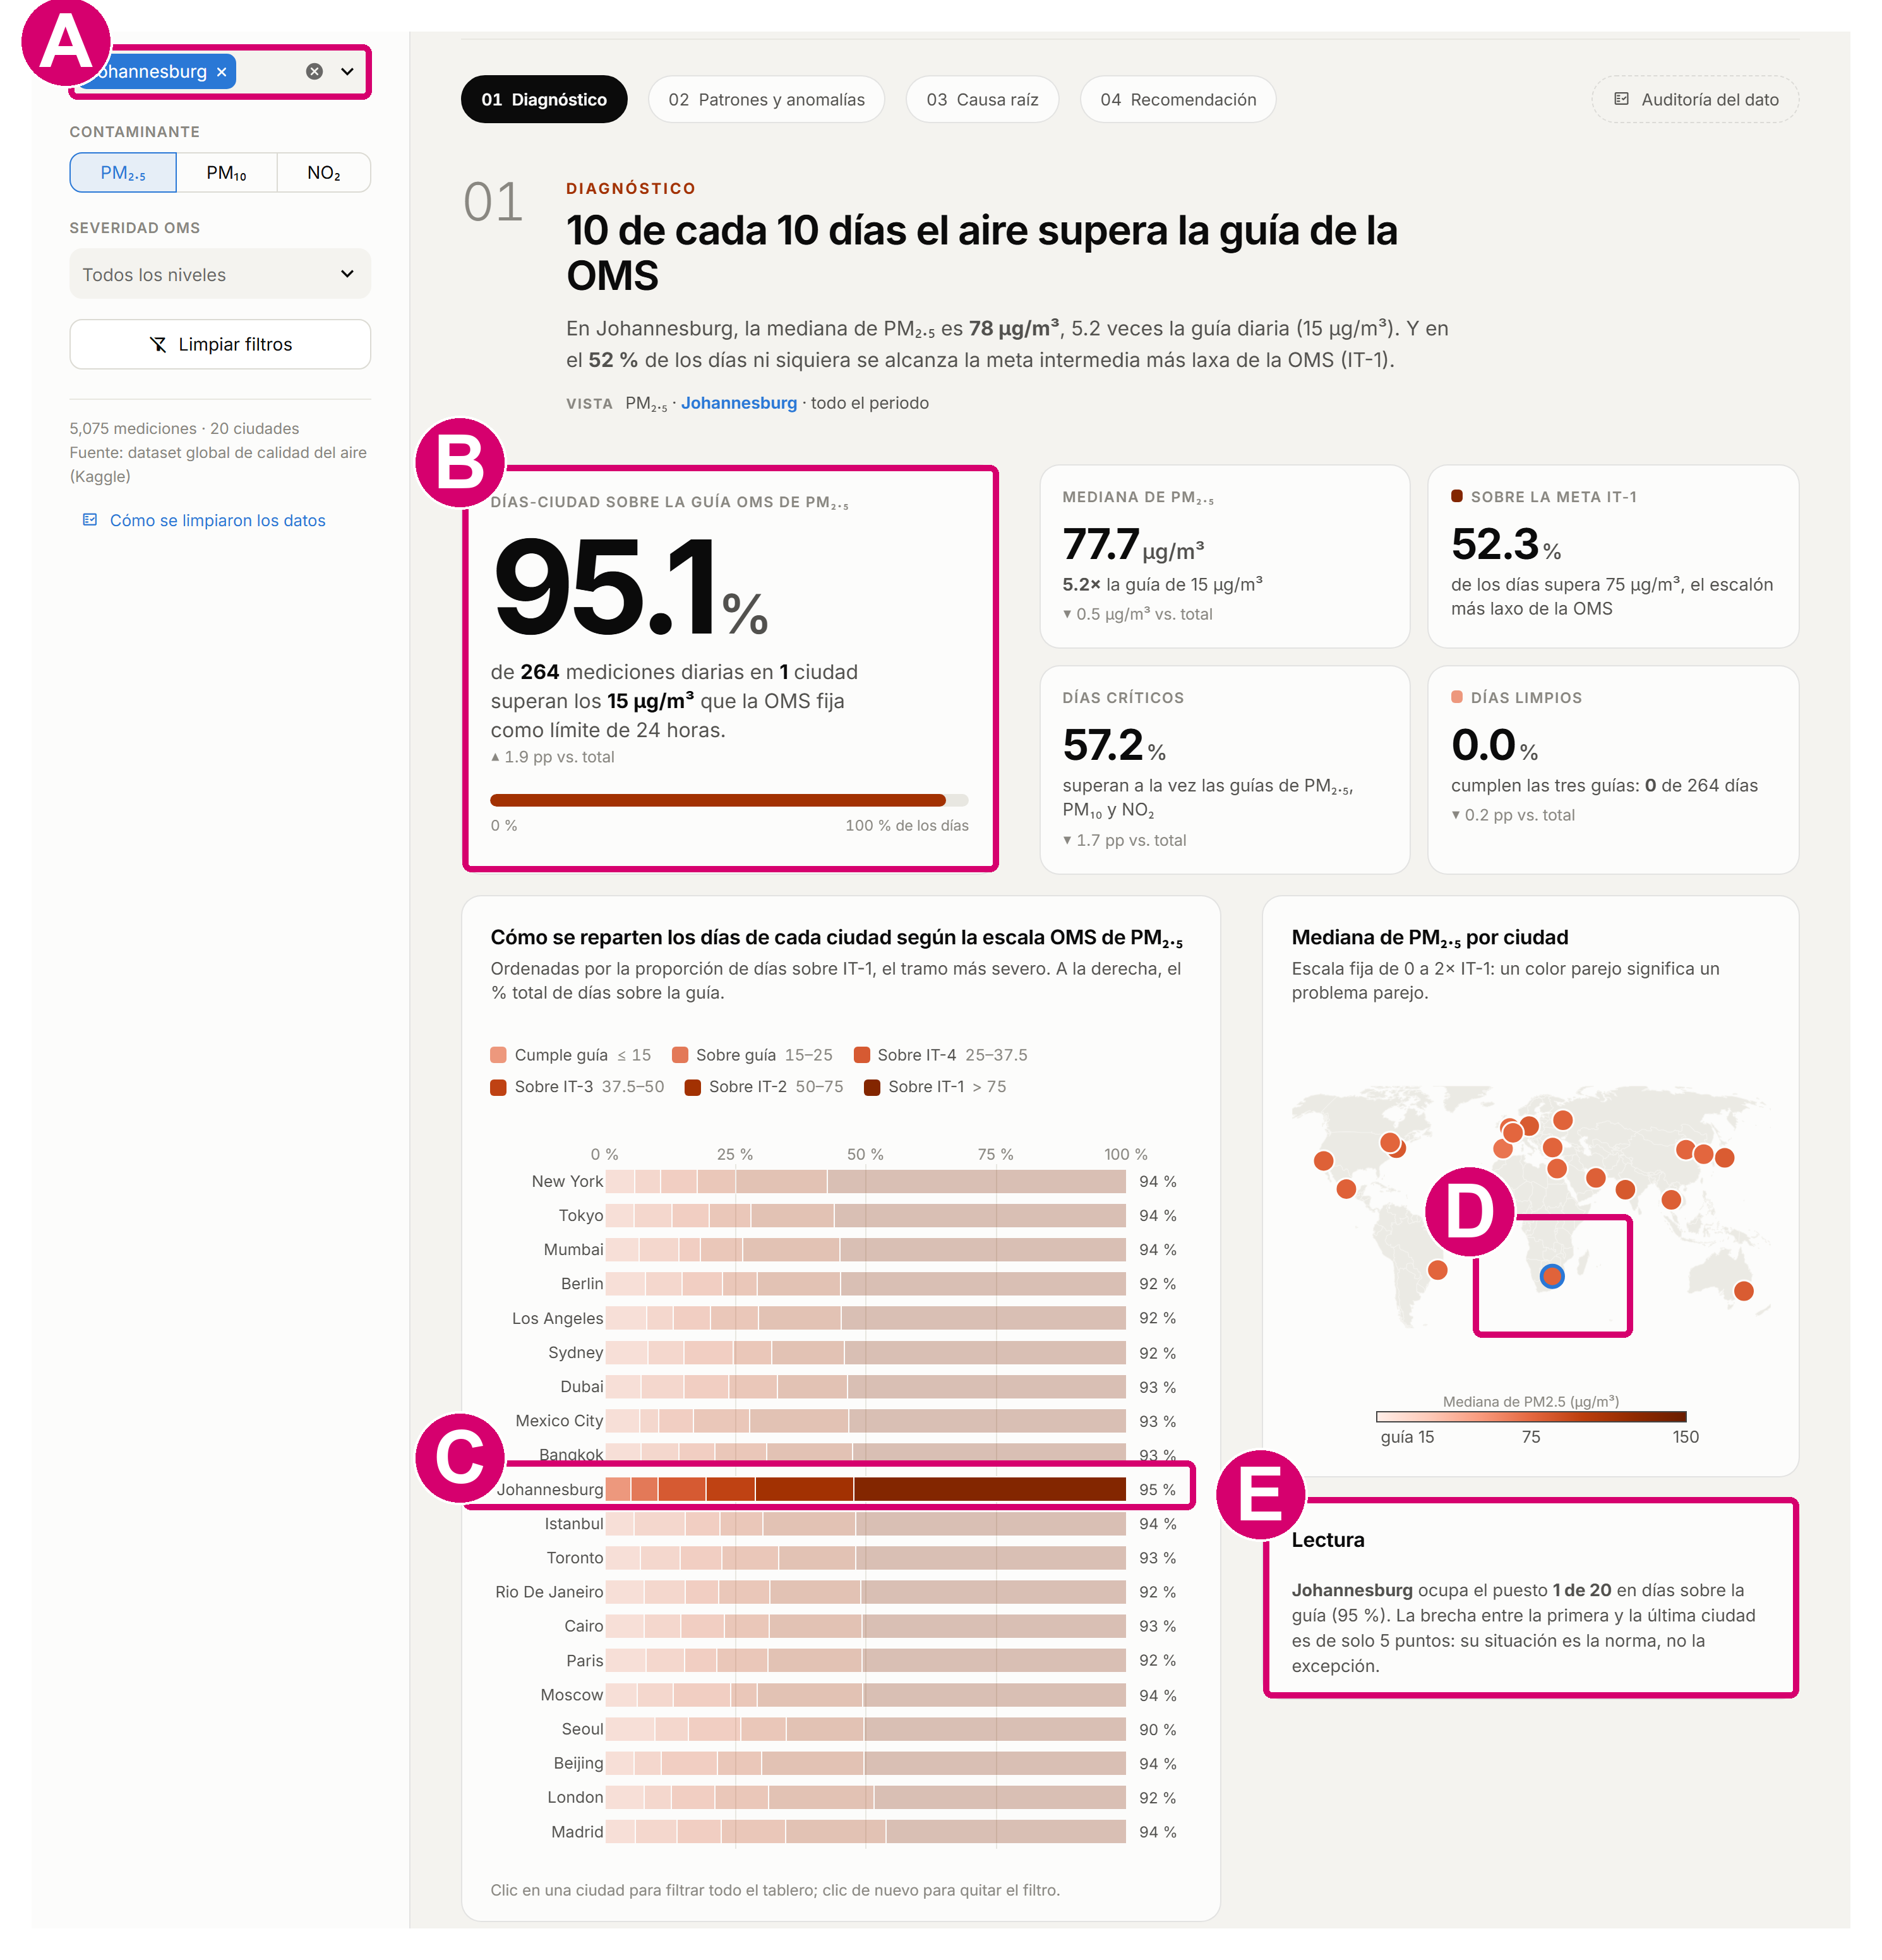
\includegraphics[width=\linewidth]{fig9_dash_diagnostico.png}
  \caption{Capítulo 01 (Diagnóstico) con Johannesburg seleccionada. (A)~Filtro de ciudad sincronizado con el clic. (B)~KPI principal con su delta frente al total. (C)~Barra resaltada y resto atenuado (foco $+$ contexto). (D)~Ciudad marcada en el mapa con un anillo azul. (E)~Texto de lectura generado para la selección.}
  \label{fig:dash_diag}
\end{figure}

\textbf{Caso 2: patrones y anomalías.} El calendario ciudad$\times$semana, la serie con media móvil de 7 días y las barras mensuales (Fig.~\ref{fig:dash_patrones}) muestran la ausencia de estacionalidad: el porcentaje de días sobre la guía oscila entre 90\% (mayo) y 96\% (junio). Los episodios (días por encima del percentil 95 de su ciudad) suman 263, y la racha más larga sobre IT-1 dura 7 días (Bangkok). Además, el 35.8\% de las lecturas presenta PM$_{2.5}>$PM$_{10}$, físicamente imposible y repartido de forma pareja entre ciudades, lo que apunta a un problema sistemático de calibración y es coherente con la correlación casi nula entre ambas variables de la Sección~IV: se interpreta como una anomalía del dato, no como independencia.

\begin{figure}[htbp]
  \centering
  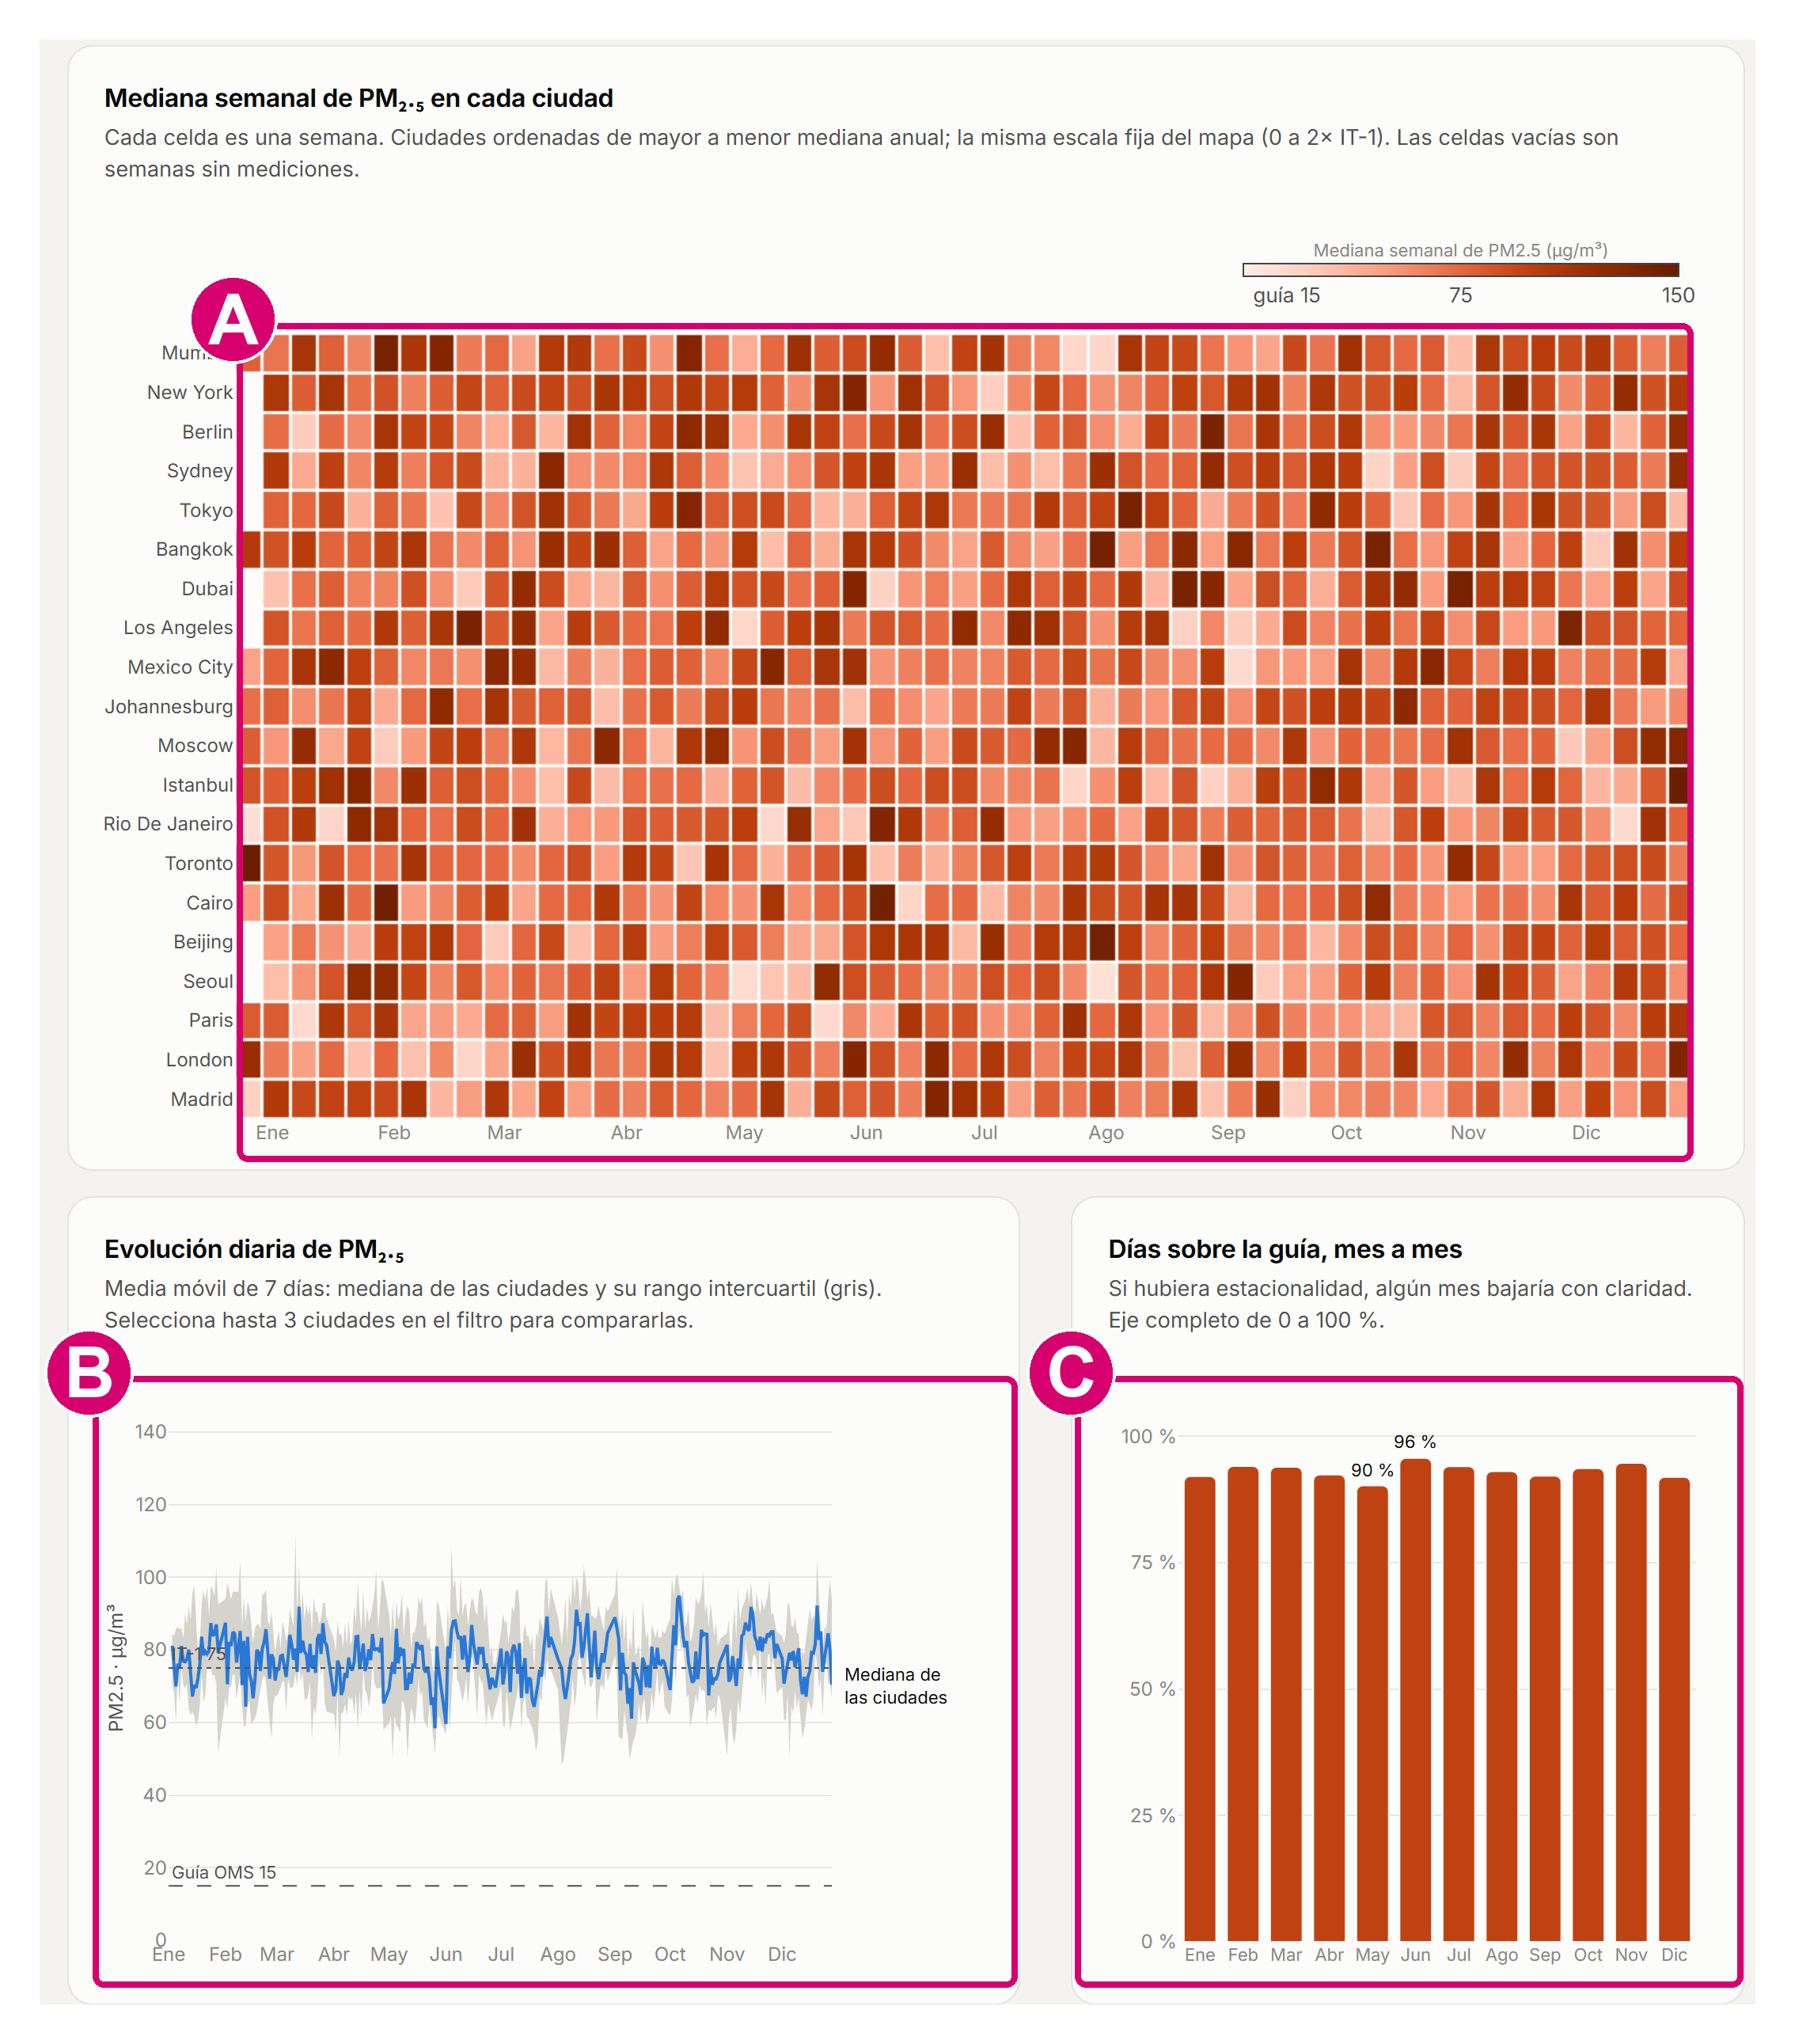
\includegraphics[width=\linewidth]{fig10_dash_patrones.png}
  \caption{Capítulo 02 (Patrones y anomalías). (A)~Calendario de la mediana semanal por ciudad con escala fija. (B)~Media móvil de 7 días con banda intercuartílica y línea de guía OMS. (C)~Porcentaje de días sobre la guía por mes, con eje completo de 0 a 100\%.}
  \label{fig:dash_patrones}
\end{figure}

\textbf{Caso 3: causa raíz.} El marcador de hipótesis (Fig.~\ref{fig:dash_causa}) exige a cada factor superar dos filtros: significancia estadística ($p<0.05$) y relevancia práctica (efecto mayor al 10\% de la mediana, 7.8~\textmu g/m$^3$). Los seis factores quedan descartados. Ciudad presenta el mayor efecto (15~\textmu g/m$^3$) pero con $p=0.85$, y el panel lateral lo señala explícitamente: una diferencia grande sin significancia no es evidencia. La conclusión, una contaminación de fondo y constante, se obtiene sin tablas de coeficientes.

\begin{figure}[htbp]
  \centering
  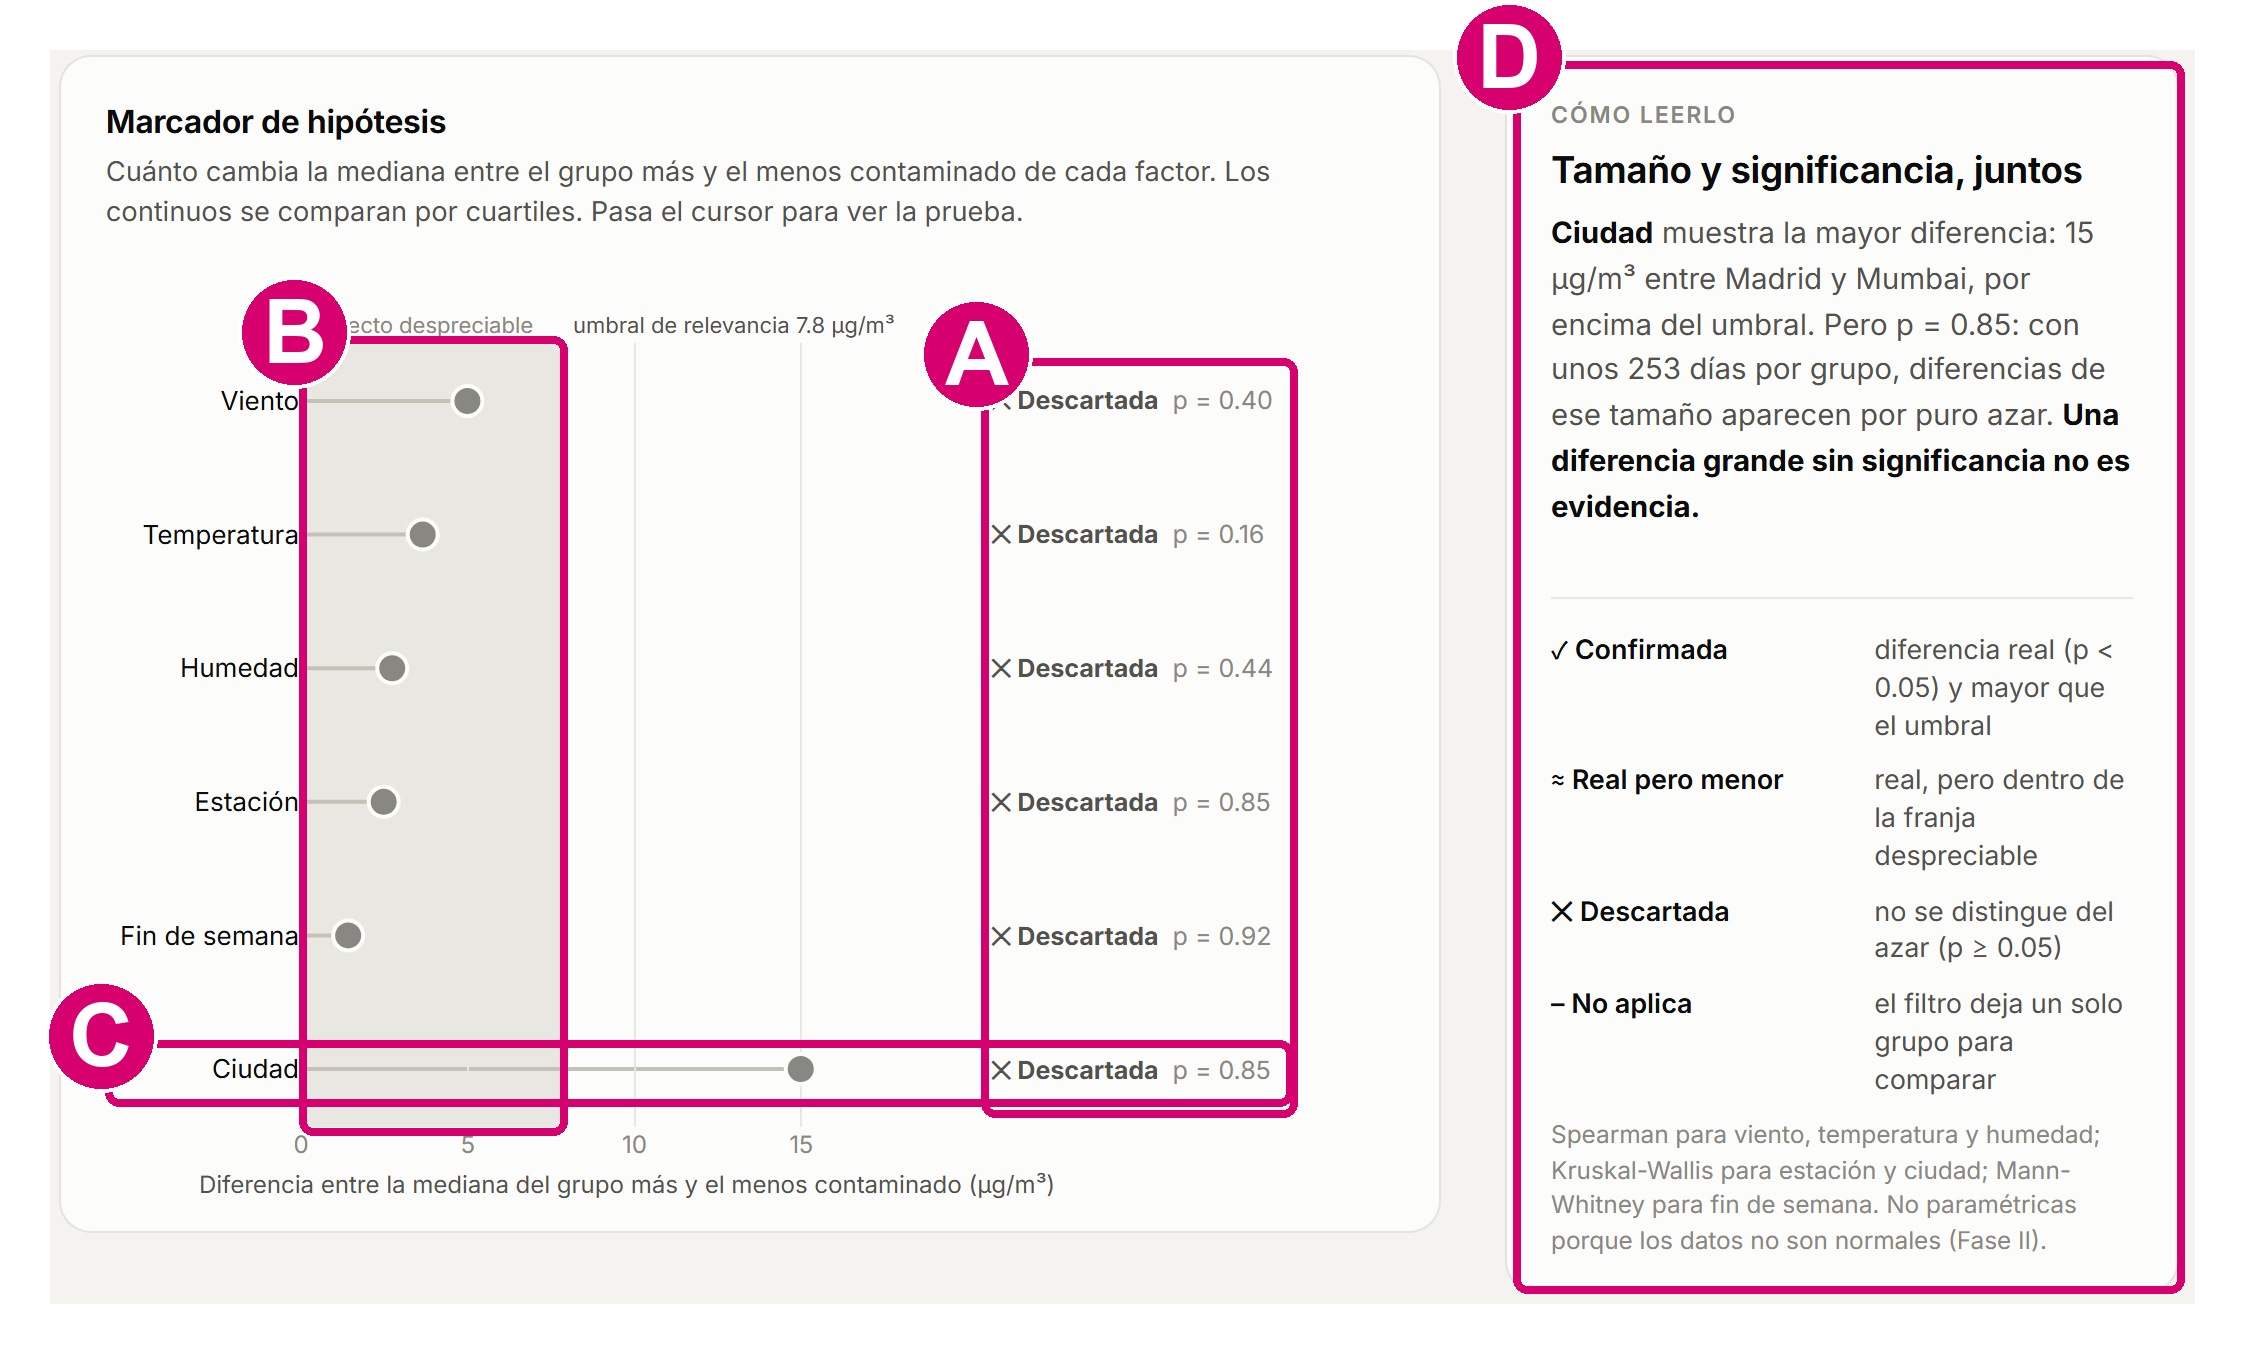
\includegraphics[width=\linewidth]{fig11_dash_causa.png}
  \caption{Capítulo 03 (Causa raíz). (A)~Veredicto con icono y valor $p$ por factor. (B)~Franja de efecto despreciable y umbral de relevancia. (C)~Ciudad: efecto grande pero no significativo. (D)~Guía de lectura de los cuatro veredictos y de las pruebas no paramétricas utilizadas.}
  \label{fig:dash_causa}
\end{figure}

\textbf{Caso 4: recomendación y simulación.} Con el deslizador en $-40\%$ (Fig.~\ref{fig:dash_reco}), los días que cumplen la guía pasan de 7\% a 14\% y los días sobre IT-1 de 52\% a 17\%, pero ninguna meta se alcanza: la hoja de ruta indica que se requiere recortar al menos 50\% para IT-1 y 90\% para la guía. Así el usuario descubre por sí mismo por qué la respuesta debe ser por etapas. El supuesto de recorte proporcional se declara en pantalla porque el Capítulo~03 no halló factores externos que modulen la contaminación.

\begin{figure}[htbp]
  \centering
  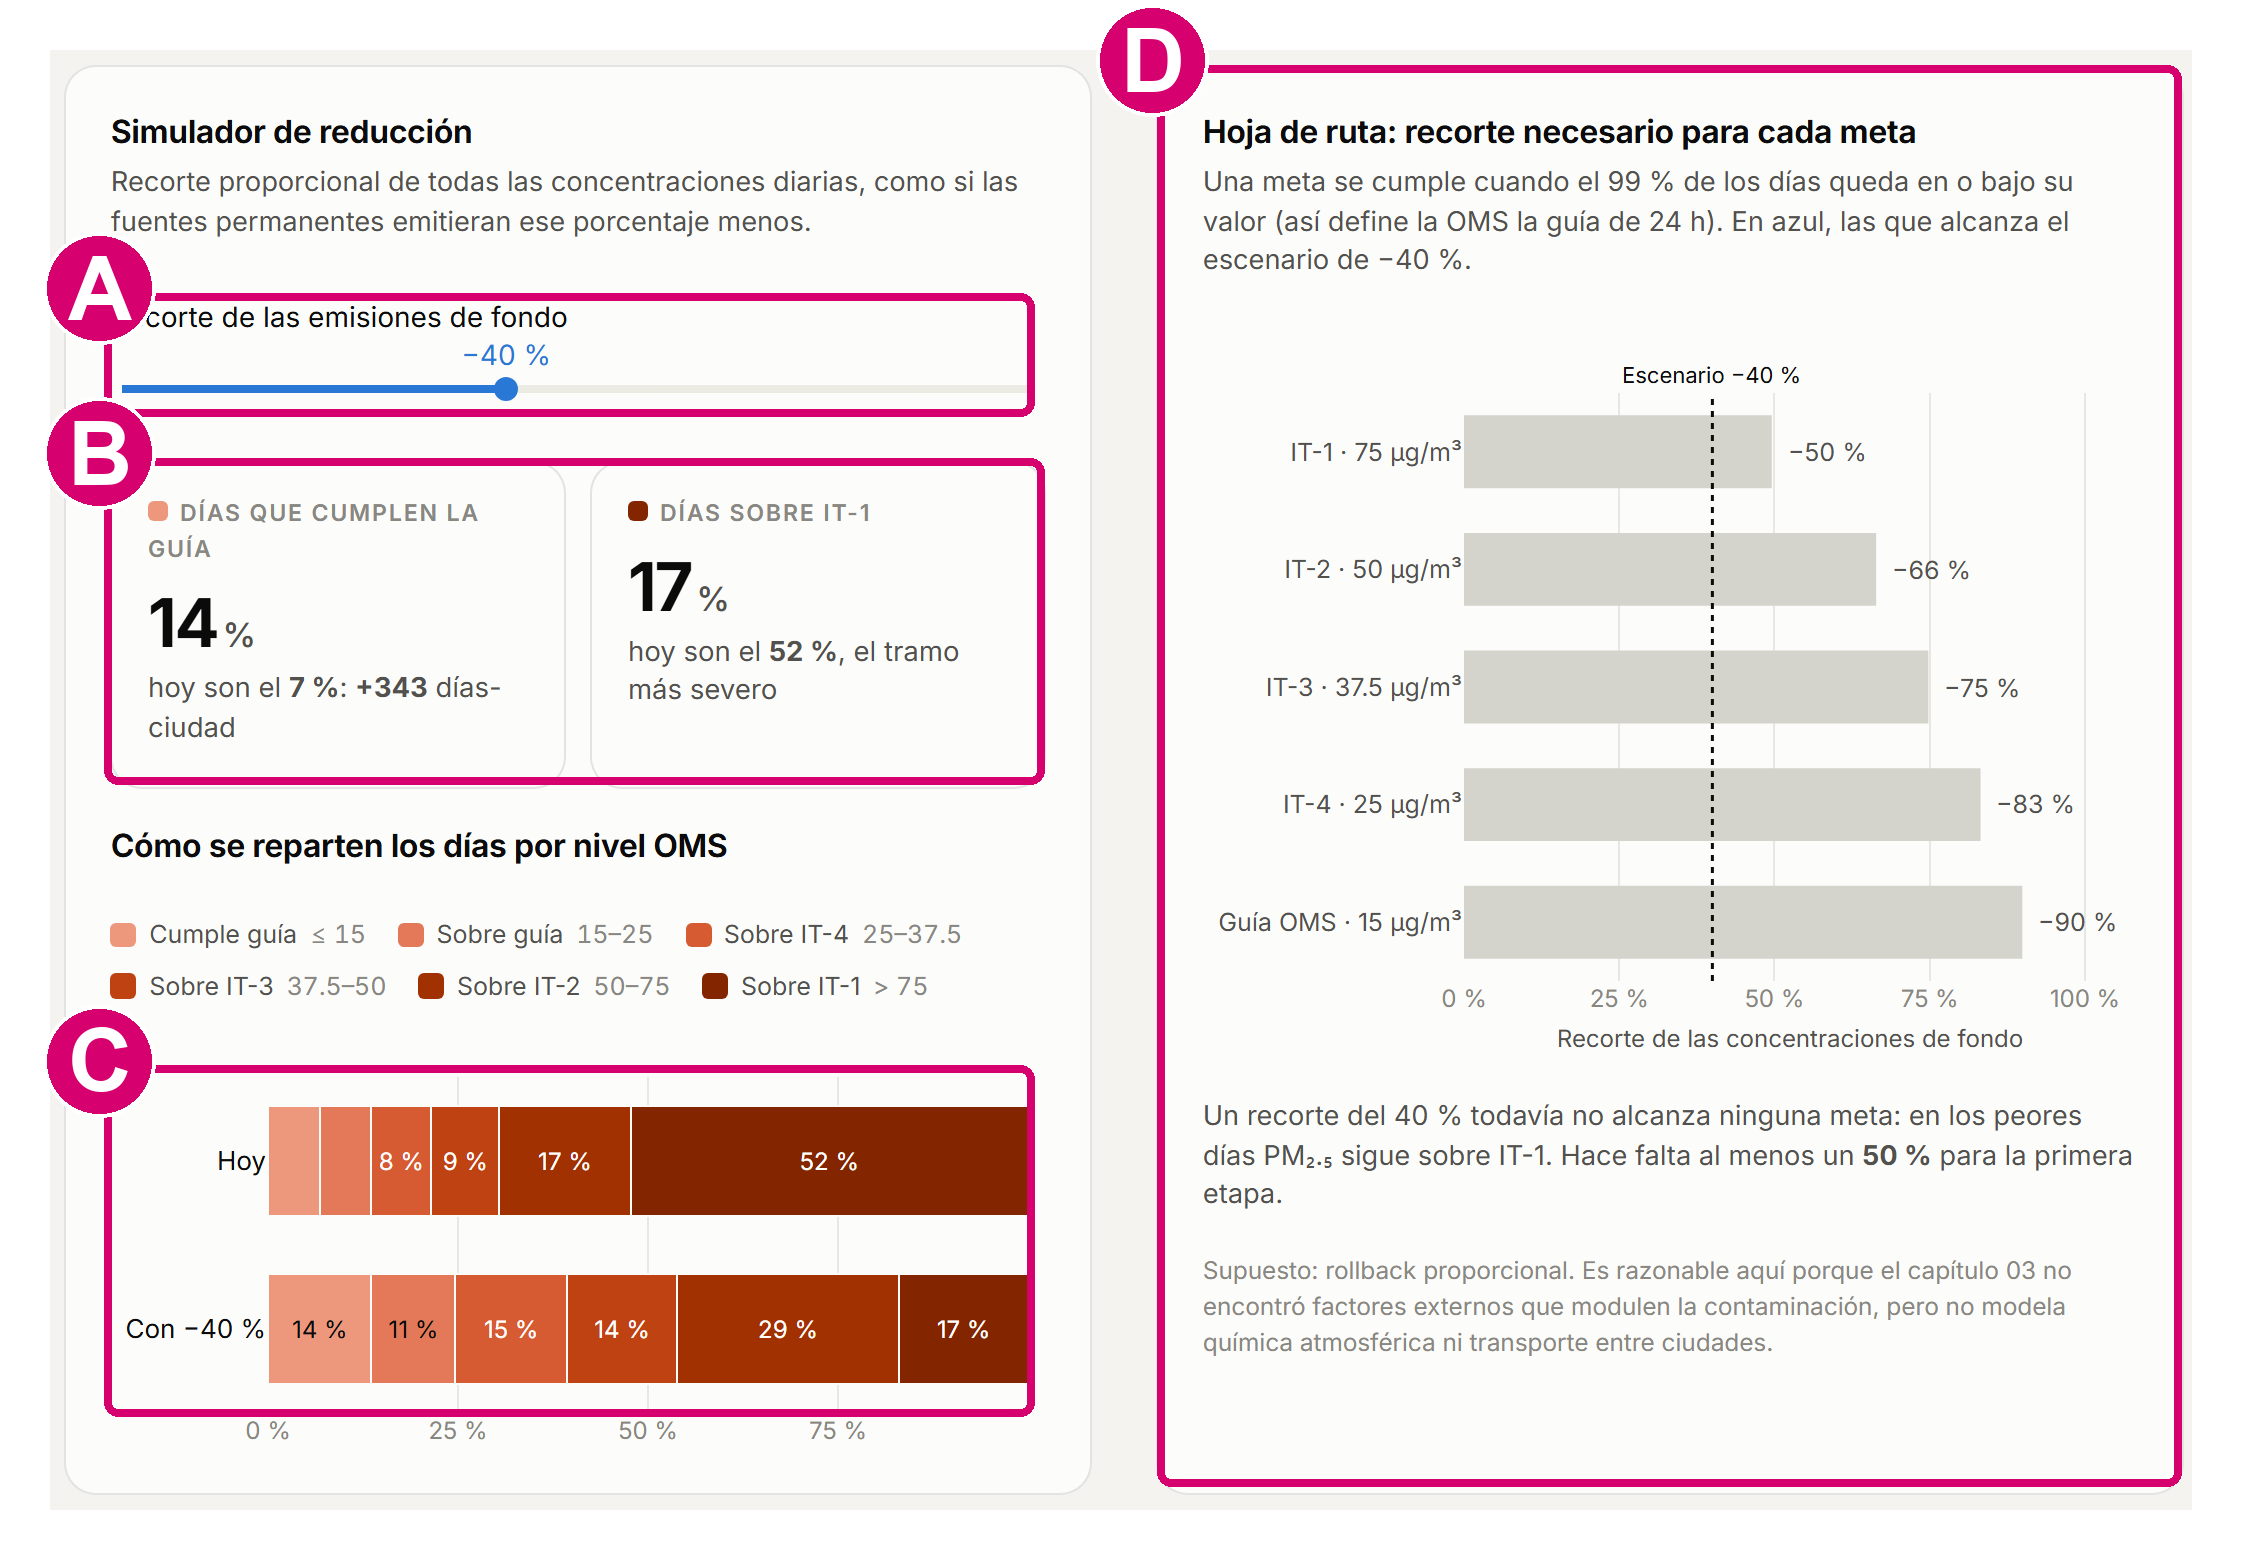
\includegraphics[width=\linewidth]{fig12_dash_recomendacion.png}
  \caption{Capítulo 04 (Recomendación) con un escenario de $-40\%$. (A)~Deslizador de recorte. (B)~KPI reactivos con su valor actual. (C)~Distribución por nivel OMS, hoy y con el escenario, con la misma rampa de severidad. (D)~Hoja de ruta con el recorte necesario por meta y la línea del escenario.}
  \label{fig:dash_reco}
\end{figure}

\begin{thebibliography}{99}

\bibitem{OMS2021}
World Health Organization, \emph{WHO global air quality guidelines: particulate matter (PM2.5 and PM10), ozone, nitrogen dioxide, sulfur dioxide and carbon monoxide}, Geneva, Switzerland: World Health Organization, 2021.

\bibitem{McKinney2010}
W. McKinney, ``Data Structures for Statistical Computing in Python,'' in \emph{Proc. 9th Python Sci. Conf. (SciPy 2010)}, Austin, TX, USA, 2010, pp. 56--61.

\bibitem{Pedregosa2011}
F. Pedregosa \emph{et al.}, ``Scikit-learn: Machine Learning in Python,'' \emph{J. Mach. Learn. Res.}, vol. 12, pp. 2825--2830, 2011.

\bibitem{Tukey1977}
J. W. Tukey, \emph{Exploratory Data Analysis}, Reading, MA, USA: Addison-Wesley, 1977.

\bibitem{Rousseeuw1993}
P. J. Rousseeuw and C. Croux, ``Alternatives to the Median Absolute Deviation,'' \emph{J. Amer. Statist. Assoc.}, vol. 88, no. 424, pp. 1273--1283, 1993.

\bibitem{Wickham2014}
H. Wickham, ``Tidy Data,'' \emph{J. Statist. Softw.}, vol. 59, no. 10, pp. 1--23, 2014.

\bibitem{Waskom2021}
M. Waskom, ``seaborn: statistical data visualization,'' \emph{J. Open Source Softw.}, vol. 6, no. 60, p. 3021, 2021.

\bibitem{Rivas2022}
D. L. L. Rivas y E. A. M. Portillo, ``Evaluación de la calidad del aire y su impacto en la salud de poblaciones urbanas,'' Tesis de Grado, Universidad Evangélica de El Salvador, San Salvador, El Salvador, 2022.

\bibitem{Little2019}
R. J. A. Little and D. B. Rubin, \emph{Statistical Analysis with Missing Data}, 3rd ed., Hoboken, NJ, USA: John Wiley \& Sons, 2019.

\bibitem{Munzner2014}
T. Munzner, \emph{Visualization Analysis and Design}, Boca Raton, FL, USA: CRC Press, 2014.

\bibitem{Cleveland1984}
W. S. Cleveland and R. McGill, ``Graphical Perception: Theory, Experimentation, and Application to the Development of Graphical Methods,'' \emph{J. Amer. Statist. Assoc.}, vol. 79, no. 387, pp. 531--554, 1984.

\bibitem{Mackinlay1986}
J. Mackinlay, ``Automating the Design of Graphical Presentations of Relational Information,'' \emph{ACM Trans. Graph.}, vol. 5, no. 2, pp. 110--141, 1986.

\bibitem{Bertin2011}
J. Bertin, \emph{Semiology of Graphics: Diagrams, Networks, Maps}, Madison, WI, USA: Univ. of Wisconsin Press, 2011 (trad. de la ed. francesa de 1967).

\bibitem{Shneiderman1996}
B. Shneiderman, ``The Eyes Have It: A Task by Data Type Taxonomy for Information Visualizations,'' in \emph{Proc. IEEE Symp. Visual Languages}, Boulder, CO, USA, 1996, pp. 336--343.

\bibitem{Brehmer2013}
M. Brehmer and T. Munzner, ``A Multi-Level Typology of Abstract Visualization Tasks,'' \emph{IEEE Trans. Vis. Comput. Graphics}, vol. 19, no. 12, pp. 2376--2385, 2013.

\bibitem{Sweller1988}
J. Sweller, ``Cognitive Load During Problem Solving: Effects on Learning,'' \emph{Cognitive Sci.}, vol. 12, no. 2, pp. 257--285, 1988.

\bibitem{Tufte2001}
E. R. Tufte, \emph{The Visual Display of Quantitative Information}, 2nd ed., Cheshire, CT, USA: Graphics Press, 2001.

\bibitem{Ware2012}
C. Ware, \emph{Information Visualization: Perception for Design}, 3rd ed., Waltham, MA, USA: Morgan Kaufmann, 2012.

\bibitem{Harrower2003}
M. Harrower and C. A. Brewer, ``ColorBrewer.org: An Online Tool for Selecting Colour Schemes for Maps,'' \emph{Cartographic J.}, vol. 40, no. 1, pp. 27--37, 2003.

\bibitem{Few2013}
S. Few, \emph{Information Dashboard Design: Displaying Data for At-a-Glance Monitoring}, 2nd ed., Burlingame, CA, USA: Analytics Press, 2013.

\bibitem{Furnas1986}
G. W. Furnas, ``Generalized Fisheye Views,'' in \emph{Proc. ACM CHI}, Boston, MA, USA, 1986, pp. 16--23.

\bibitem{Heer2012}
J. Heer and B. Shneiderman, ``Interactive Dynamics for Visual Analysis,'' \emph{Commun. ACM}, vol. 55, no. 4, pp. 45--54, 2012.

\end{thebibliography}

\end{document}
